\chapter{再帰\hspace{-3mm}}

この章では再帰について学びます。ターゲットとなるプログラムは次のものです。

\begin{lstlisting}
[:letrec, 
 [[:fact,
   [:lambda, [:n], [:if, [:<, :n, 1], 1, [:*, :n, [:fact, [:-, :n, 1]]]]]]], 
 [:fact, 3]]
\end{lstlisting}

まずは準備として、$\mu$SchemeRの機能を少し拡張しましょう。

\section{条件式}

次のようなif式で条件を扱えるようにします。

\begin{lstlisting}
[:if, [:>, 3, 2], 1, 0]
\end{lstlisting}

if式の評価はif式から条件、真節、偽節を取得し、条件の評価値が真であれば真節を評価し、偽であれば偽節を評価し、その値を返します。

if式を評価するプログラムを上のとおり書いていきましょう(後で使う{\tt letrec}も合わせて一緒に定義しています)。

\begin{lstlisting}
def special_form?(exp)
  lambda?(exp) or 
     let?(exp) or 
     letrec?(exp) or 
     if?(exp)
end

def eval_special_form(exp, env)
  if lambda?(exp)
    eval_lambda(exp, env)
  elsif let?(exp)
    eval_let(exp, env)
  elsif letrec?(exp)
    eval_letrec(exp, env)
  elsif if?(exp)
    eval_if(exp, env)
  end
end

def eval_if(exp, env)
  cond, true_clause, false_clause = if_to_cond_true_false(exp)
  if _eval(cond, env)
    _eval(true_clause, env)
  else
    _eval(false_clause, env)
  end
end

def if_to_cond_true_false(exp)
  [exp[1], exp[2], exp[3]]
end

def if?(exp)
  exp[0] == :if
end
\end{lstlisting}

if式で分岐するために論理値のリテラルを導入します。
{\tt :true}, {\tt :false}は(Rubyの)true, falseとして解釈するよう大域環境に加えます。

\begin{lstlisting}
$boolean_env = 
    {:true => true, :false => false}
$global_env = [$primitive_fun_env, $boolean_env]
\end{lstlisting}

条件式で扱えるよう、組み込み関数に不等号、等号の演算子を加えます。

\begin{lstlisting}
$primitive_fun_env = {
  :+  => [:prim, lambda{|x, y| x + y}],
  :-  => [:prim, lambda{|x, y| x - y}],
  :*  => [:prim, lambda{|x, y| x * y}],
  :>  => [:prim, lambda{|x, y| x > y}],
  :>= => [:prim, lambda{|x, y| x >= y}],
  :<  => [:prim, lambda{|x, y| x <  y}],
  :<= => [:prim, lambda{|x, y| x <= y}],
  :== => [:prim, lambda{|x, y| x == y}],
}
$global_env = [$primitive_fun_env, $boolean_env]
\end{lstlisting}

\section{再帰}

これで準備が出来ました。いよいよ再帰を見ていきます。次のプログラムを実行してみましょう。

\begin{lstlisting}
[:let, 
 [[:fact,
   [:lambda, [:n], [:if, [:<, :n, 1], 1, [:*, :n, [:fact, [:-, :n, 1]]]]]]], 
 [:fact, 0]]
\end{lstlisting}

1が表示されましたか。では次のプログラムはどうでしょう。

\begin{lstlisting}
[:let, 
 [[:fact,
   [:lambda, [:n], [:if, [:<, :n, 1], 1, [:*, :n, [:fact, [:-, :n, 1]]]]]]], 
 [:fact, 1]]
\end{lstlisting}

エラーになりました。この違いは何でしょう。{\tt :let}を評価すると{\tt :fact}をλ式の値であるクロージャに束縛します。このクロージャの環境には{\tt :fact}は含まれていない点に注意しましょう。{\tt [:fact 1]}として関数適用するとクロージャ中の環境を用いて評価します。評価を進め、if式で偽となると{\tt :fact}を評価しますが、先に述べたようにこの環境には{\tt :fact}は含まれていないためエラーとなるのです(図\ref{fig:let})。すなわち、関数として定義しようとした式の中でその関数の名前を使うにはlet式では不十分であることが分かります。

\begin{figure}[htbp]
\begin{center}
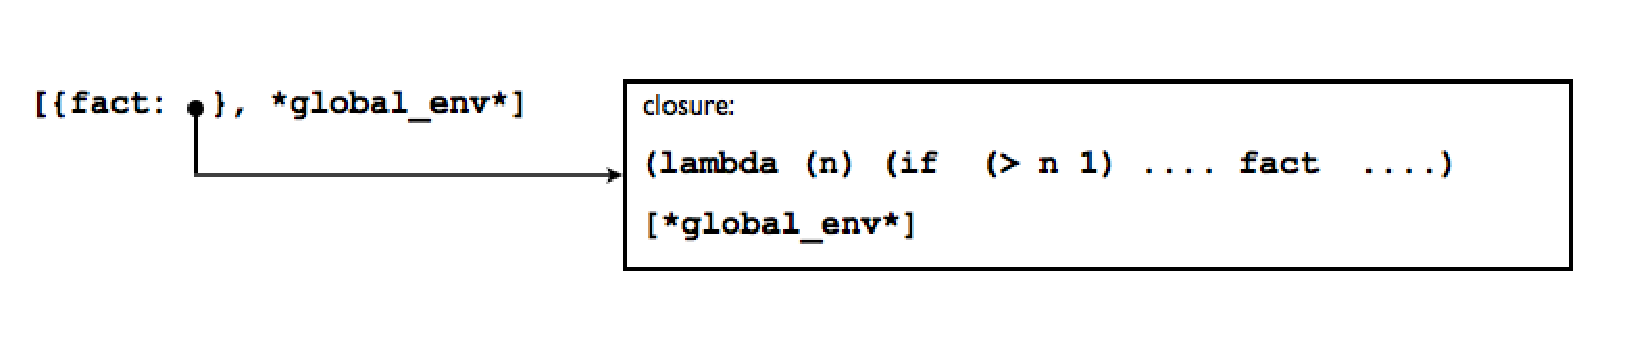
\includegraphics[width=140mm]{images/let.eps}
\end{center}
\caption{{\tt [:fact 1]}評価時の環境のようす。λ式評価時の環境に{\tt fact}がないため、クロージャ内の環境には{\tt fact}は存在せず、{\tt [:fact 1]}でクロージャ中の{\tt fact}を参照しようとするとエラーになる。}
\label{fig:let}
\end{figure}

これを解決するためにはどうすれば良いでしょう。問題は、先に述べたように、{\tt :lambda}を評価してクロージャを作るときに{\tt :fact}が束縛されていないため、返されたクロージャを関数適用に用いると、その中の{\tt :fact}が評価できない点にあります。すなわち、作られるクロージャ中の環境に、それが出来た後で束縛しようとしている{\tt :fact}が含まれている必要があるのです。

これを解決するために、少しトリッキーなことを行います。アイデアは、λ式
を評価しクロージャを作成するときに環境として予め、パラメータ(ここで
は{\tt :fact})の領域を確保しておくことです。ただし、それを束縛する値はまだ定
まっていないので、ダミーの
値を入れておきます(図\ref{fig:letrec}(a))。このとき、パラメータは評価さ
れないためダミーの値でも問題にはなりません。λ式を評価してもλ式の中は
評価されずにクロージャとして返されるためです。λ式の評価値であるクロー
ジャが得られたら、先ほどのパラメータをダミーの値からその値に束縛するよ
うに変更します。(図\ref{fig:letrec}(b))
これでパラメータを評価すると、そのパラメータを環境とし
て含むクロージャを得ることが出来ます。得られた環境を使ってletrec式のボ
ディ{\tt [:fact, 1]}を評価すると(図\ref{fig:letrec}(c))、λ式内の{\tt :fact}
を所望どおり参照することが出来ます。

\begin{figure}[htbp]
\begin{center}
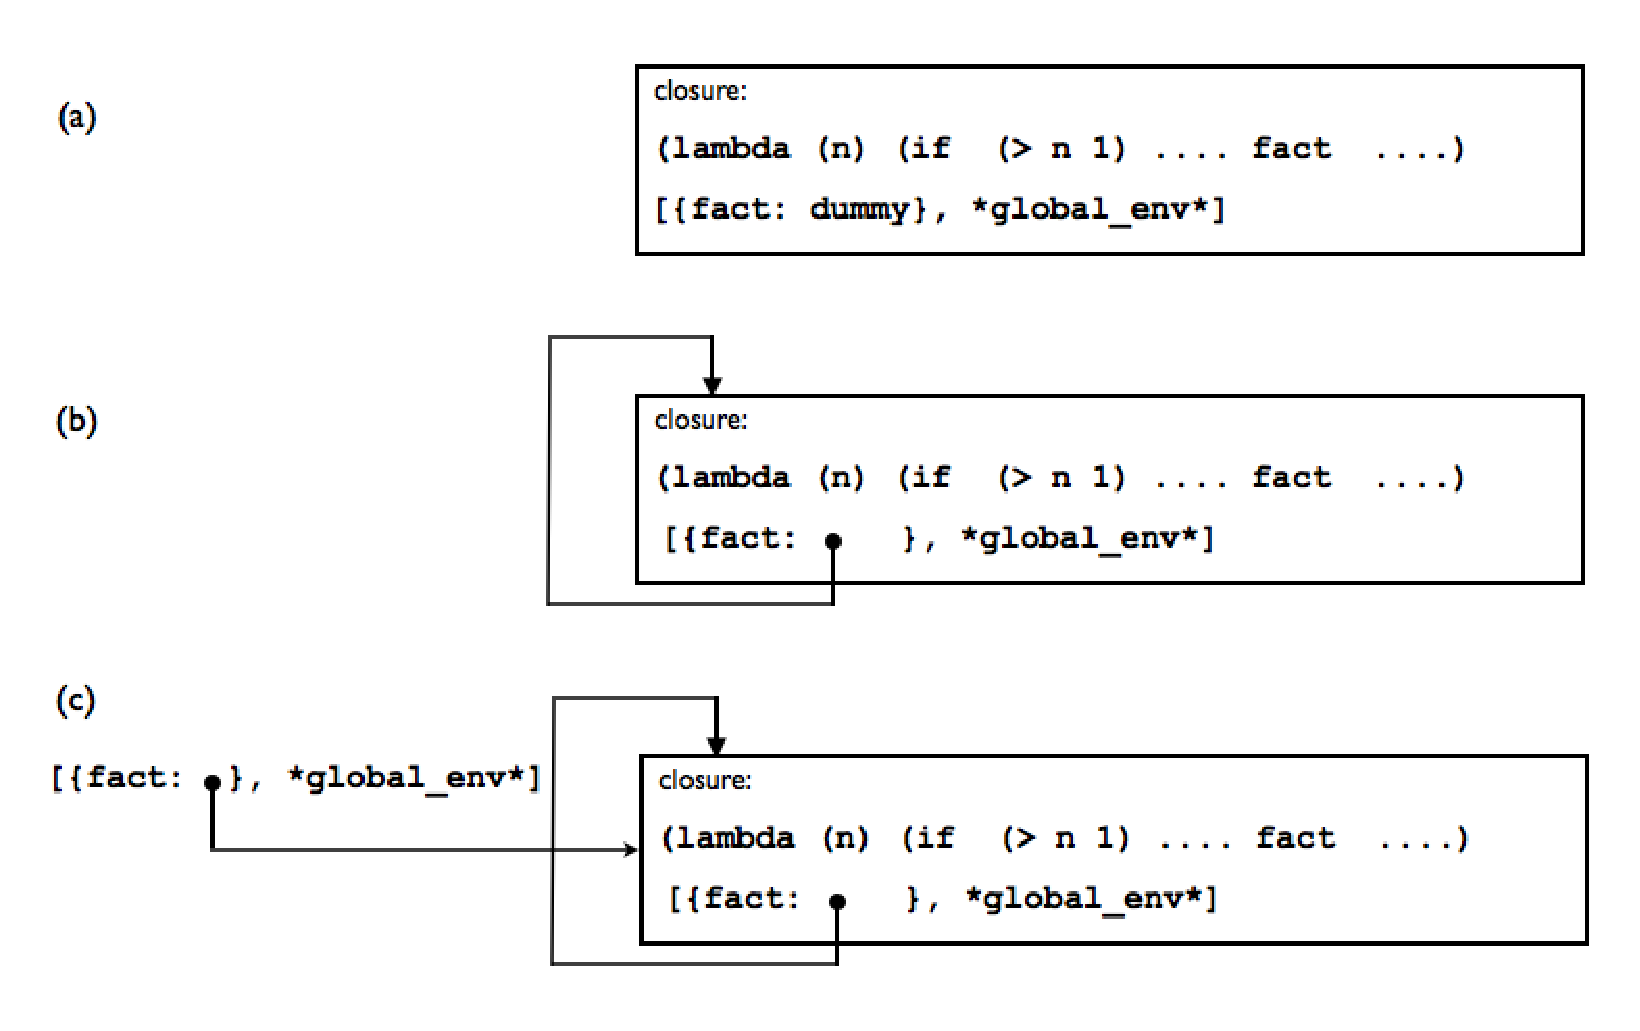
\includegraphics[width=140mm]{images/letrec.eps}
\end{center}
\caption{(a)λ式の評価時の環境に{\tt fact}をダミー値{\tt dummy}に束縛しておき、(b)得られたクロージャの環境の{\tt fact}をクロージャ自身に束縛することで、(c){\tt [:fact 1]}でクロージャの環境内の{\tt fact}が参照可能となる}
\label{fig:letrec}
\end{figure}


以上の機構を実装した再帰を扱う{\tt letrec}を導入します。

\begin{lstlisting}
def eval_letrec(exp, env)
  parameters, args, body = letrec_to_parameters_args_body(exp)
  tmp_env = Hash.new
  parameters.each do |parameter| 
    tmp_env[parameter] = :dummy
  end
  ext_env = extend_env(tmp_env.keys(), tmp_env.values(), env)
  args_val = eval_list(args, ext_env)
  set_extend_env!(parameters, args_val, ext_env)
  new_exp = [[:lambda, parameters, body]] + args
  _eval(new_exp, ext_env)
end

def set_extend_env!(parameters, args_val, ext_env)
  parameters.zip(args_val).each do |parameter, arg_val|
    ext_env[0][parameter] = arg_val
  end
end

def letrec_to_parameters_args_body(exp)
  let_to_parameters_args_body(exp)
end

def letrec?(exp)
  exp[0] == :letrec
end
\end{lstlisting}

それでは、実際に試してみましょう。

\begin{lstlisting}
exp =
  [:letrec, 
   [[:fact,
     [:lambda, [:n], [:if, [:<, :n, 1], 1, [:*, :n, [:fact, [:-, :n, 1]]]]]]], 
   [:fact, 3]]
puts _eval(exp, $global_env)
\end{lstlisting}

正しく、6が表示されましたね。

\section{純粋関数型言語 -- 代入はどこへ?}

おめでとうございます。あなたは、この時点で関数型言語で必要な全ての要素
を学んだと言えます。ただし“最小限の範囲内で”、という限定付きです。今
までに学んできたプログラミング言語は、純粋関数型言語(pure functional
language)と言われ、代入と言った副作用の無い言語です。状態が変わらない、
そもそも状態すら持たないために、変数を、それを束縛している値で入れ替え
ても問題ありません。最適化ではインライン展開と言われる手法です。関数呼
び出しを減らすことが出来るためそれに関わるコストを削減できます。関数呼
び出し時に、環境のスタックを積み上げたことを思い出して下さい。それが不
要になります。もしくは、どの順序で評価してもその値は変わらないため、そ
れぞれを並列に処理することができます。最近、関数型言語が見直されるよう
になってきたのは、このような背景が多分にあります。

そうは言っても手続き型言語で代入を多用している方にとっては、本当に代入
なしで複雑な処理を記述できるのか疑問に思われることでしょう。大丈夫です。
実は、今まで書いてきたRubyのプログラムも簡単に代入なしで書くことが出来
ます。本質的に代入が必要なのは、たった一ヶ所、set\_extend\_env!で使わ
れているハッシュへの代入のみです\footnote{関数名の最後の!は、quoteの
略で、Schemeでは一般的に副作用がある関数の最後にクオート文字!をつけてこ
れを区別しています。この慣習に倣いました。}。他の箇所では引数で渡された配列の中
を代入などにより変更していません。したがってこれ以外の代入は、let式相当の機能
で置き換えても問題ありません(Rubyにはlet式相等の機能がありませんが...)。

本書で考えるプログラミング言語にはあえて代入は導入しません。下手に代入があるとそれに頼ってしまうことがあるからです。新しい関数型言語の考え方に慣れるためにこの言語で色々と処理を書いて見てください。


\section{関数型言語と再帰 -- for文はどこへ?}

再帰は関数型言語にとって大きな意味を持ちます。手続き型言語のfor文など
ループに相当する重要な制御構文です。関数型言語の特徴は、データ構
造に着目して再帰的に処理をすることが多い点です。

実は今回の対象としているプログラミング言語も、数字など基本的な式を組
み合わせて一つのプログラムとなるように設計されています。これ
を式の構成に関する帰納法と呼びます。{\tt eval\_let}などの中で、評価すべ
きプログラムを構成している要素に分け、それぞれの要素に対して再帰的に
{\tt eval}していることを確認してみて下さい。

また、先の例では階乗を求めるプログラムfactを使いました。これも見方を変
えると再帰的に定義された整数に従った構成に関する帰納法とも言えます。整
数
は、0という整数が存在すること、またある整数が存在したとき+1したものが次に大きな整数として
定義されます。この定義に従い、0のときの解を示し、またある整数が与えら
れた時、それより一つ小さい整数の解を用いて求めるものを定義することで、全て
の場合の解を求めることができます。

その他にもまだ扱っていませんが、リストは空リストであるか、リストに先頭
の要素を加えたものである、と再帰的に定義されます。一般的なリスト
を扱う関数はこの定義に従い、与えられたリストが空リストであった場合の処
理と、与えられたリストの最初の要素に対する処理を記載し、残りのリストは
再帰を使って定義します。わかりづらいと思いますので、\ref{chap:extend}章
のp. \pageref{sec:list}のリストの項目(特に{\tt length}関数)を見てからも
う一度この文章を読んで見てください。


\section{まとめ}

この章では次のことを学びました。

\begin{itemize}
\item 再帰関数を実現するための方法
\item 再帰関数の評価値であるクロージャは、その中の環境でクロージャ自身を参照する。
\item これまでに作成してきた$\mu$SchemeRは代入のような副作用がない純粋関数型言語である
\item 手続き言語のループに相当するものを関数型言語では再帰を用いる
\end{itemize}

% % \begin{boxnote}
% {\bf コラム: {\tt letrec}の意味} \\

% 以下、少し高度な話になりますので初めての方は読み飛ばしていただいてかまいません。ここでは{\tt letrec}の意味について少しお話しします。

% 前に、下のプログラムはエラーになることをお話ししました。これは、{\tt :lambda}の中の{\tt :fact}が何も束縛していないためです。
% \begin{lstlisting}
% [:let, 
%  [[:fact,
%    [:lambda, [:n], [:if, [:<, :n, 1], 1, [:*, :n, [:fact, [:-, :n, 1]]]]]]], 
%  [:fact, 1]]
% \end{lstlisting}
% それでは、その{\tt fact}をもう一度同じで{\tt fact}に束縛する、すなわちそのままコードを置き換えると、どうなるでしょう。
% \begin{lstlisting}
%    [[:let, 
%      [[:fact,
%        [:lambda, [:n], 
%         [:if, [:<, :n, 1], 1, 
%          [:*, :n, 
%           [:let, 
%            [[:fact,
%              [:lambda, [:n], [:if, [:<, :n, 1], 1, [:*, :n, [:fact, [:-, :n, 1]]]]]]],
%            [:fact, [:-, :n, 1]]]]]]]], 
%      [:fact, 1]]
% \end{lstlisting}
% 今度は1が表示されたと思います。ただし{\tt [:fact, 2]}を評価すると、今度は一番内側の{\tt :lambda}の中の{\tt fact}が何も束縛していないので、エラーになります。しかし、もう一度今度は一番内側の{\tt :fact}を同じように展開してやると、{\tt [:fact, 2]}まで計算できるようになります。

% このようにn回展開したコードを$\Phi^{n}_{fact}(\emptyset)(x)$とおくと、
% \begin{eqnarray}
%   \Phi^{n}_{fact}(\emptyset)(x)=\left\{ \begin{array}{ll}
%       x! & (0 \leq x < n) \\
%       エラー & (x \geq n) \\
%     \end{array} \right.
% \end{eqnarray}
% となります。

% これを無限回展開したものを、$\Phi^{*}_{fact}$とおくと、これは実質上、factを計算することが出来ます。
% %% $\Phi_{fact}$の話をして、$\Phi^{*}_{fact}(\Phi^{*}_{fact}) = \Phi^{*}_{fact}が成り立つ不動点の話をして、letrecが不動点を求める演算子であるということを言いたい...
% % \end{boxnote}
